% vim: foldmethod=marker foldcolumn=3

\vspace{-4pt}
{

\noindent
\begin{tabular*}{0.999\textwidth}
    {|c | p{0.827\textwidth}< {\centering} |}
    \hline
    {\songti 论文题目} & {\songti 面向数据中心网络的流量分析与故障检测} \\ 
    \hline
\end{tabular*}
\indent

\begin{mdframed}[everyline=true]

% {{{ 选题
\section{选题依据及意义}

数据中心被目前的企业中所广泛采用, 大型的数据中心甚至承载着公司的服务系统. 其中
服务器与服务器之间几乎完全是通过现代网络所连接. 用户对网络性能的要求日益扩大,
一些微小故障, 很可能会造成用户体验的下降, 特别是在某些交互敏感的场合.
服务的质量必须得到保证. 可是对于庞大的系统, 各种问题的发生是无法避免的. 我们
只能更快, 更精准的解决问题, 以此将故障的危害降到最低. 这也是对新时代的检测调试
工具的挑战.


面对大型复杂数据中心的调试以及错误, 如果仍然使用简陋的单机调试手段,
例如ping, tracerout, 也许可以解决问题, 但其代价与耗时, 是无法满足运营要求的.
进而, 许多公司提出了自己的方案, 甚至为自己搭建的集群开发出一套相匹配的网络调试工具.


\section{研究目标和主要内容(含论文(设计)提纲)}

在数据中心网络(DCN)中, 众多网络设备运行过程中的故障在所难免, 及时发现故障并确定 
故障位置成为DCN网络运维的重要组成部分. 本课题参照微软提出的Everflow故障检测方案,
设计实现一款面向数据中心网络的流量分析与故障检测工具.

为了解决现实存在的数据中心的网络异常问题, 利用现有交换机的"Match and Mirror"
机制, 将特定的数据包进行镜像. 分析镜像后的数据包, 以达到对网络中存在问题的检测.

本次设计中, 将会基于通用的处理器平台, 关注于DCN中环路的检测, 结果保存, 预警,
数据展示, 探针构造几个方面. 初步实现Everflow功能的基础上, 进行了简单的改进完善:

\begin{itemize}
    \setlength\itemsep{0.1em}
    \item 加入了对快慢路径两种不同的分析方案;
    \item 在分析时, 多处使用hash数据结构来加快查找, 以加快处理速度;
    \item 采用B/S架构, 管理员通过浏览器即可进行操作.
\end{itemize}
% }}}

% {{{  文献综述
\section{文献综述: 国内外研究现状,发展动态}

不论是学校还是企业, 许多都设立了自己的数据中心,
有关数据中心的网络故障检测, 都提出了自己的 见解与考量.
对于更为大型的数据中心网络, 更是有人提出了集学校公司之力, 共同开发系统,
不断的部署 与完善.

经过对国内外近期文献的查阅, 我发现,
这些系统或是工具可以按照不同角度进行分类. 在主动性方面,
有主动探测故障的, 有被动触发, 还有使用日志记录来查看的; 在网络层次方面,
有些在数据包层面, 有些 则专注于数据流层面; 根据部署位置不同,
也可以分为在交换机部署, 在终端部署, 两者均进行部署; 在 使用范围上,
有些适合于通用平台, 有些只能适用于某个特定厂商; 在处理上,
有些拥有流水线来处理结果, 有些则是简单的排除错误; 按工具性质来看,
有些属于调试小工具, 专注于某个方面, 也不需要一直在线,
有些则是属于系统级别的服务工具, 为整个DCN所使用的服务, 需要一直在线;
而后在错误处理上, 有些 可以借助控制设备自动进行处理,
而有些则需要向管理员预警, 手动进行处理. 以下为各个方案的一些特点 介绍.

Planck: \upcite{rasley2014planck} SDN的出现使得自己调节的网络得以实现, 这样
的网络可以实时监控, 并能立即对重要的事件例如拥塞做出迅速反应.
但是目前的监控机制 需要数百毫秒来重新探测全局网络, 对于实时的错误,
这样的延迟是很致命的, 这篇2014年 的论文提出了新颖的网络测量架构,
使用端口镜像的机制来提取网络信息. 但是可以在相当
短的时间内对网络信息进行获取. 而且不会对网络造成太大的影响.

LossRadar: \upcite{li2016lossradar} 属于有针对性的工具,
着重介绍有关丢包的抓取 问题. 虽然只是检测丢包,
但是这也足够成为一个检测系统了, 这个工具可以在较快的时间
内抓取单独的丢包以及他们的详细信息. 他需要在交换机上部署,
但是并不需要很多的流量 和带宽. 也基于它开发了一些应用程序.

Cherrypick: \upcite{tammana2015cherrypick} 一个可扩展的简单的轨迹追踪技术
目前的数据轨迹追踪需要负担大量数据积累的开销,
或是在数据平面大量资源的消耗, 交换机规则或是数据包头部的探查.
核心思想是挑选链接, 这些链接是表示数据包端到端 路径的关键,
并在到达目的地的路上将其嵌入数据包头部. 通过使用最新的头部标示技术,
它只需要很少的交换机规则即可,

SDN traceroute: \upcite{agarwal2014sdn} 使用具有了SDN功能的设备, 不过只要
支持OpenFlow1.0的设备即可.
他可以通过SDN支持的网络中的任意数据包来确定路径,
这个路径使用SDN支持的转发机制, 而且并不需要修改转发规则.
可以探测任意的以太网 数据包的转发行为,
以及交换机和控制器逻辑中的调试问题.

PathDump: \upcite{tammana2016simplifying}使用了较为不同的方法,
仔细划分了边缘 设备与网络元素之间的调试任务.
利用边缘设备的资源进行网络调试的简约工具. 并且可以 支持大量网路调试问题.
需要的资源较少, 而且在较细的时间粒度调试.

Pingmesh: \upcite{guo2015pingmesh}
这个系统已经在微软的数据中心部署了超过4年, 他的理念很简单,
就是想要在任意时刻获取任意两台服务器的延迟信息. 因此, 他的目标就是
去定义一个网络延迟检测和分析系统, 他也需要为所有的服务器产生延迟信息,
因为延迟数据 属于基础信息, 能够帮助我们更好的管理网络,
以及解决网络中的问题. 这项服务也必须 长期在线, 并保证稳定性.
他可能是最不需要关心路由器等设备的一个方案了, 对于整个系统 来说,
知道延迟就是目标, 在实现时, 主要借助了ping的思想,
所有服务器要从中心控制器 下载文件, 进行延迟探测后传回中心服务器.
他借助了微软自己开发了存储系统, 也实现了 数据处理流水线.
相比于之后提出的Everflow, 他更像是微软的第一代产品, 稳定而强大.

NetSight: \upcite{handigol2014know}, 这是一个完全记录网络历史的工具.
在文章中, 介绍了如何使用packet
histories(每个包的整条记录)来简化网络的调试.
为了展示\texttt{packet\ histories}的作用, 以及实现上的可行性,
创造了\texttt{NetSight}, 一个可扩展的平台,
允许程序简便的检索网络的历史状况. 在\texttt{NetSight}上, 有4个程序:
可交互的网络调试器, 实时的监视器, 一个历史记录器, 一个分级分析器.
在一个现代的多核服务器上,
\texttt{NetSight}可以处理历史包在10G/s的链接中. 对于更大的 网络,
它可以通过增加服务器或是硬件 或是交换机的数量来扩展. 需要借助SDN,
支持Openflow的交换机才能配合工作, 由于其记录了数据包的历史, 所以
能最大程度还原当初的网络模型, 也因此会给网络带来高负荷, 性能也会损失,
当然也可以 通过增加硬件来进行提升. 这是一个与Everflow较为相似的产品,
Everflow中对其一个 重要的改进就是增加了匹配模式, 对特定的历史包生成记录,
能有效减少网络负载, 以及处理 难度.

Netography: \upcite{zhao2016netography} 这也是一种基于软件定义网络(SDN)的
一个工具, 之前的工作关注于静态检查, 被动监控, 以及活动探针,
这些依赖于控制设备以及网络 设备的抓取规则. 他定义了一个数据包行为的概念,
用以描述数据包的真实变化, 并强调对故障排除的重要性. 基于通过
由主动发送的探测器触发的副本导出分组行为和流规则的新颖方法,
提出了Netography系统, 并说明了 关于转发错误时的排除任务过程,
以及由非租户争用造成的性能下降问题.

Dissecting RTT(round trip time): \upcite{marchetta2014dissecting} 与其说他
是工具, 不如认为这一种技术, 利用单个数据包探测延迟的技术. 研究人员
与操作者经常会在监控, 故障排除, 或是其他方式访问网络路径时 测量往返时间,
因为它结合 了所有跳的过程以及转发和反向路径, 很难去衡量特定网络元素的
延迟. 在这项工作中, 我们提出了一种新的方法: 在区块中, 映射特定路径后
基于单个数据包探测往返 延迟. 使用针对中间路由器的IP Prespecified
Timestamp选项, 它可以提供慢速路径部分的往返时间 估计.
这个技术在Everflow中也被用到了, 用于探针方法测量时延.

Everflow: \upcite{greenberg2016packet} 这也是微软推出的工具,
属于数据包层面的 调试器, 该技术有两个优点, 仅需要具有``Match and
Mirror''商用交换机即可, 而且可以 自定义的发送探针来进行测试.
也在微软的数据中心部署了超过6个月. 基于数据包层面的分析
可以有效获得整个系统的信息, 环路或是丢包等的常见问题有所探讨,
并且对于一些厂商 定制的协议, 例如RDMA流量的分析上,
也能具有很强大的分析功能.

Passive Realtime Datacenter: \upcite{roy2017passive} 这是在Facebook的数据
中心上进行测试的一种方案, 他不去简单的观察异常现象,
而是考虑异常对整个系统的性能 所造成的影响. 虽然是基于这么一种简单的设想.
但其实现需要深深结合数据中心的架构. 他们开发了轻量级的包标记技术,
仅仅使用转发规则(交换机支持). 作为路径中唯一标示. 文章中对于数据包头部,
现有IPv6头部还很难寻求一份区域用于调试.

% }}}

% {{{ 方案论证

\section{方案论证}

本次毕业设计基于微软推出的设计方案Everflow\upcite{greenberg2016packet},
通过 解析数据包层面的信息 进行网络分析.
本次的系统可行性将由以下几个方面进行说明. 但请知悉, 本次毕业设计的
重点部分为分析器以及提供交互功能的控制器,
并依照控制器提供的API进行上层软件开发,
交换机的配置以及存储器的仅作简要说明, 并不影响整体设计.

而且, 本方案中只讨论了在5跳之内的数据中心结构, 假定没有NAT协议, 一条路径上的
源IP与目的IP一直保持相同, 可以根据


% {{{ 任务书内容
\subsection{任务书内容}

\textbf{任务包括:}
\begin{itemize}
    \setlength\itemsep{0.1em}
    \item 对实时采集到的数据包进行分析, 实现丢包检测,环路分析或时延异常等故障检测;
    \item 按需保存Trace数据并在必要时生成主动探测包, 以进一步确定故障位置和故障原因;
    \item 针对上述故障检测需求进行应用界面的开发, 具备统计分析, 异常报警等功能.
\end{itemize}

原始条件及数据:
\begin{itemize}
    \setlength\itemsep{0.1em}
    \item 提供用于实验开发的软硬件环境和相关设施;
    \item 提供相关的技术资料和可离线使用的流量数据;
    \item 安排相关研究生给予一定的指导和协助.
\end{itemize}

工作要求:
\begin{itemize}
    \setlength\itemsep{0.1em}
    \item 开题之前拟定详细的工作计划;
    \item 每周以书面形式报告进展情况;
    \item 遵从实验室内部工作安排;
    \item 严格按进度安排完成各阶段工作;
    \item 遇到问题及时反馈, 在解决问题的过程中提高应变能力.
\end{itemize}
% }}}

% {{{ 设计思路
\subsection{设计思路}

  下图\ref{user_flow}为程序设计图, 本次设计将参考下图进行实现. 之后进行分条
叙述.

\begin{center}
    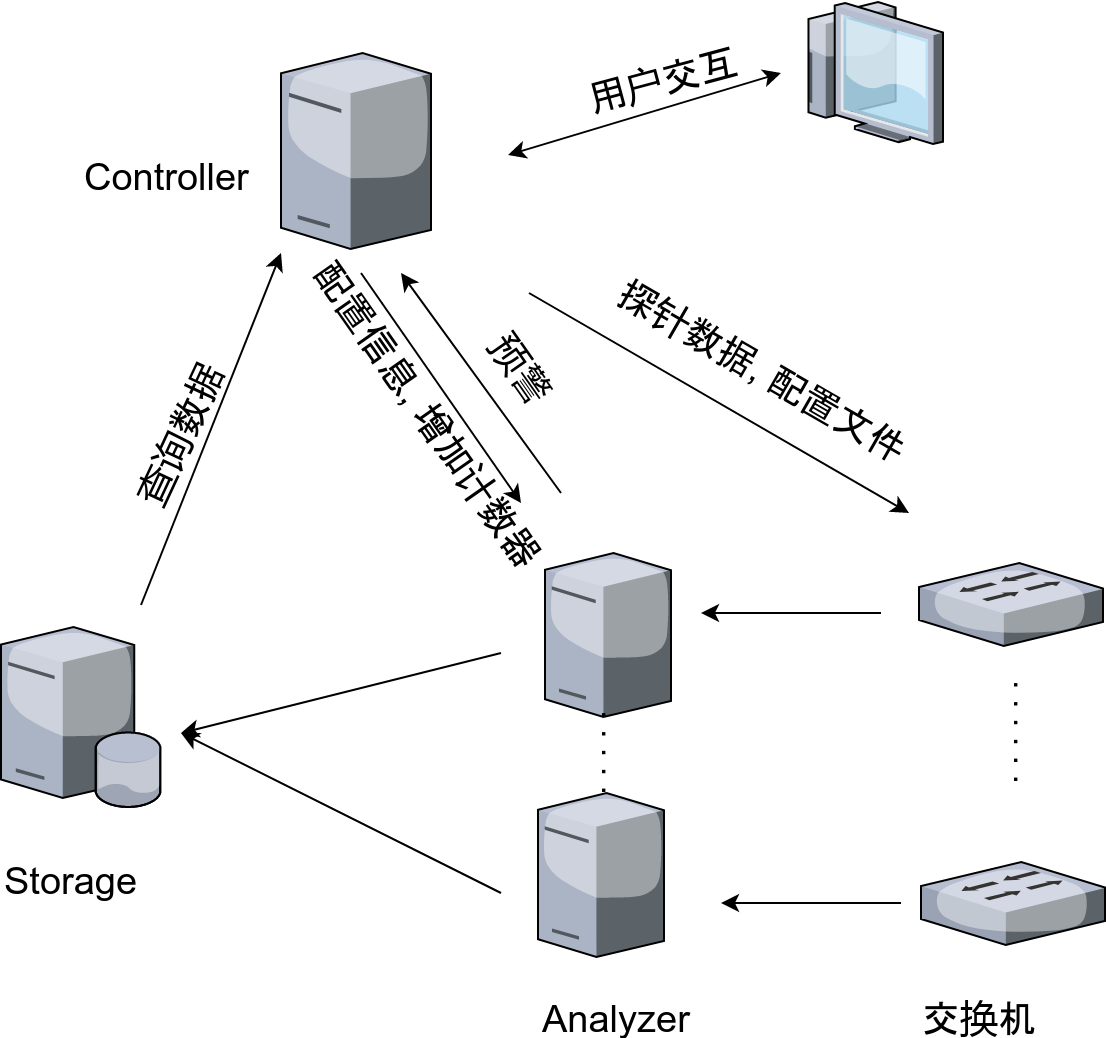
\includegraphics[width=0.7\textwidth]{../img/user_flow.png}
    \captionof{figure}{程序设计图}
    \label{user_flow}
\end{center}

\subsubsection{交换机}

  对于整个的Everflow系统, 它的输入应该是由交换机镜像后的数据包.
在\textbf{match and mirror}方面,
使用了商用交换机的SPAN(Switch port analyzer)技术,
将数据镜像并封装为GRE数据包, 关于交换机的过滤规则: 对于像BGP,
PFC以及RDMA这样的 特殊且重要的协议, 采取全部镜像的策略,
而对于TCP连接这种: 只镜像包含SYN, FIN, 和 RST的数据包,
这样既达到了探测效果, 又大大的减少分析器的开销.

\begin{center}
    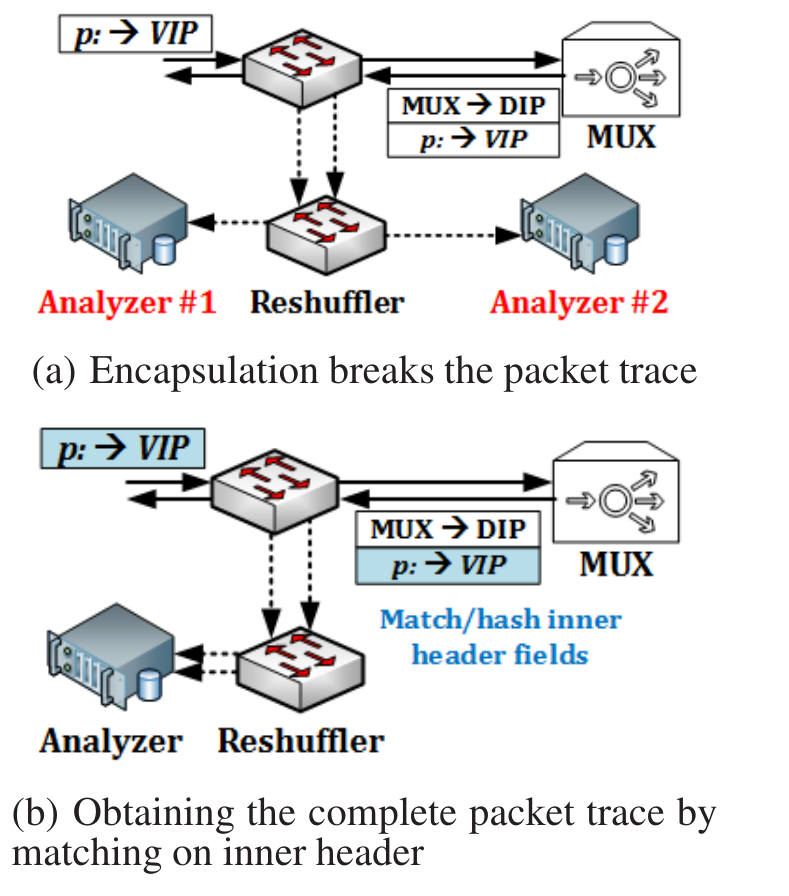
\includegraphics[width=0.7\textwidth]{../img/handle_packet_encapsulation.png}
    \captionof{figure}{packet encapsulation}
    \label{mux}
\end{center}

经过封装之后的数据包p将会传入至分析器中, 见图\ref{mux}. 但为了负载均衡,
在传入分析器之前, 还要经过一层由交换机改装好的复用器(图中MUX),
之后会再经过 洗牌器发往不同的分析器中进行分析. 这一过程虽然经过多个设备,
但这些设备均是交换机, 具有较快的处理数据包的速度.

虽然我们是在数据包层面分析问题,
但是我们想要得到的还是整个数据流传输时的情况, 这里
洗牌器这个设备承担了比较重要的工作, 具有同样5元组信息(源IP, 目的IP,
源端口, 目的端口 和协议类型)的数据包将产生同样的hash值,
通过hash值确定要传递到的分析器,
可以保证一整条数据流中的所有数据包均被传递至相同的 分析器.

\begin{center}
    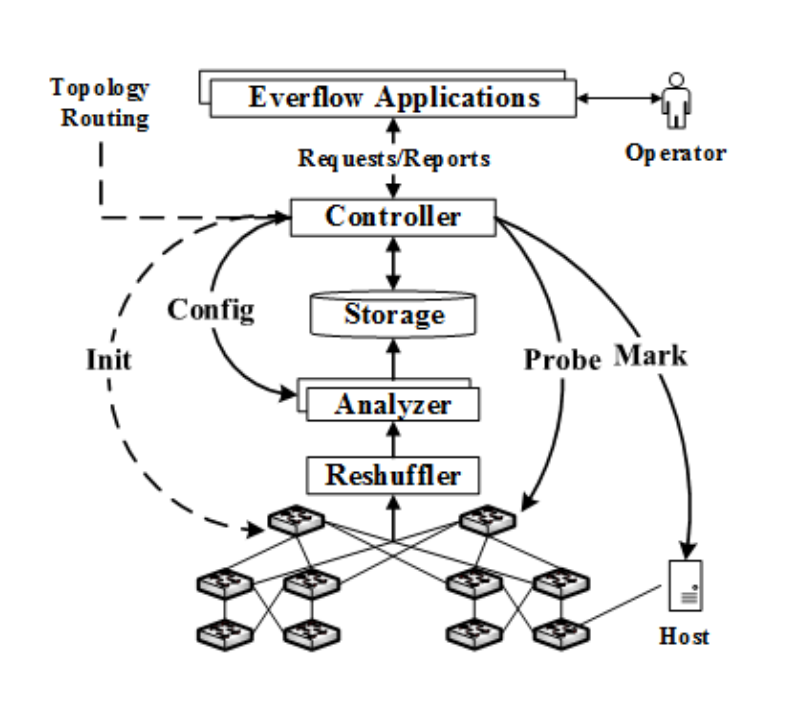
\includegraphics[width=0.8\textwidth]{../img/everflow_arch.png}
    \captionof{figure}{architecture}
    \label{arch}
\end{center}

图\ref{arch}中介绍了整个系统的结构,

\subsubsection{分析器}

  分析器读入产生的数据包后. 进行初步的处理, 而后存入存储器中供控制器使用.
在分析器中, 我们可以获得整条的数据包路径, 通过路径, 我们可以得知是否有环,
或是有丢包现象. 以及对于特定的模式进行统计, 对于探针来说也可以粗略的衡量延迟.

  以上是对分析器的简单说明, 下图\ref{analyzer_process}是具体处理过程. 首先进行
对GRE数据包的解封操作, 解封后, 使用多线程并发分析. 解封后, 具有相同标示的数据包
需要进入相同的线程中.

   分析中, 如果某一跳交换机在1s内, 没有收到接下来的报文, 即认为此次数据包已经结束,
因此, 我们需要增加定时功能. 相关算法请查看\ref{主要算法说明}中定时器的实现.

\begin{center}
    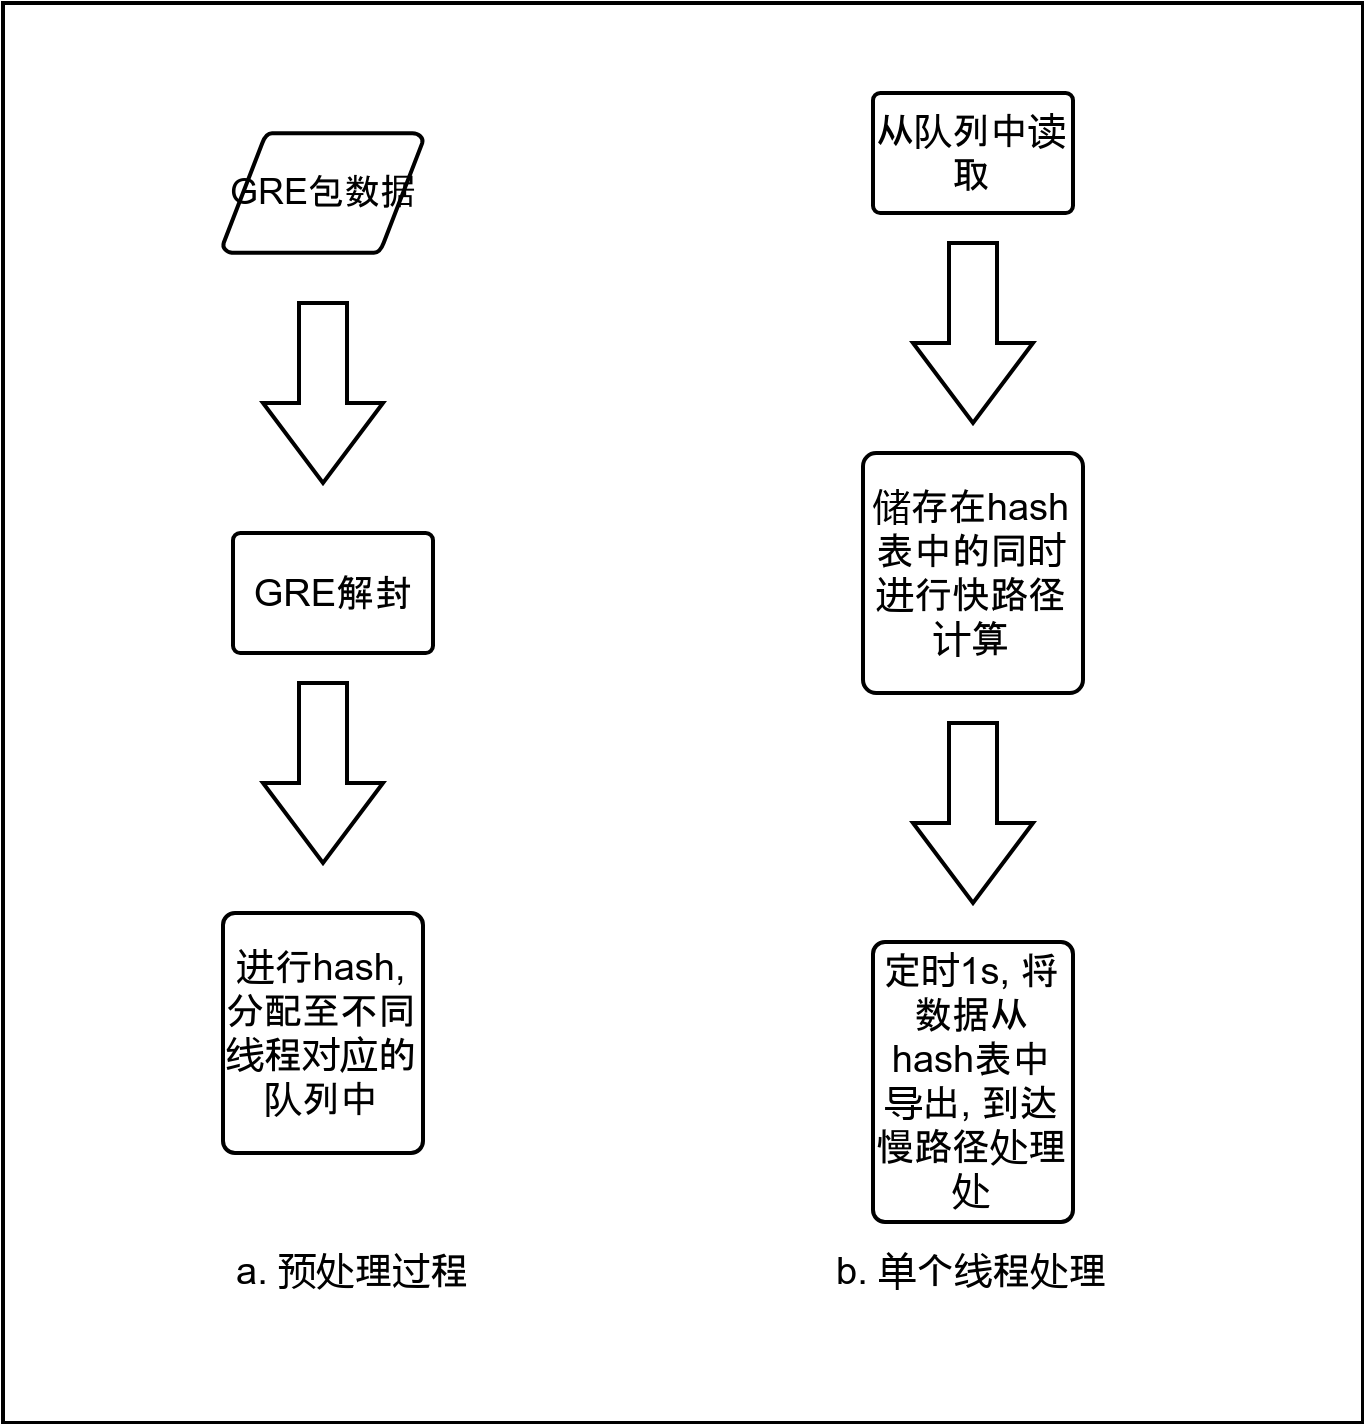
\includegraphics[width=0.8\textwidth]{../img/analyze_process.png}
    \captionof{figure}{Analyezr process}
    \label{analyzer_process}
\end{center}

\subsubsection{存储器}

分析结束后, 并不是所有的结果都要存入存储器, 只有异常行为数据流,
有debug标志的 数据流, 重要协议(BGP, PFC等)会被记录到存储器中.

\subsubsection{控制器}

控制器最重要的功能就是向外提供API接口. 除此之外, 控制器可以对分析器配置,
向交换机 中发送探针, 而后根据分析器的结果, 目前我们能够提供 的API包括
按时间查找数据流, 查询计数器的值, 添加探针, 在指定的服务器上添加标志位.

通过控制器的几个接口, 我们以此来进行上层程序设计,
本次设计中要求的使用图形界面 展示结果, 以及添加异常报警功能,
在拥有了以上的API后, 这样的功能实现起来并不困难.

具体的API将会在程序完成后随说明文档提供.


\subsubsection{有关展示界面}

下图\ref{traffic_data_show}, \ref{counter_data_show}分别展示了数据流量的显示以及
计数器结果的显示, 目前主要列出信息模块, 搜索功能会接着完善

\begin{center}
    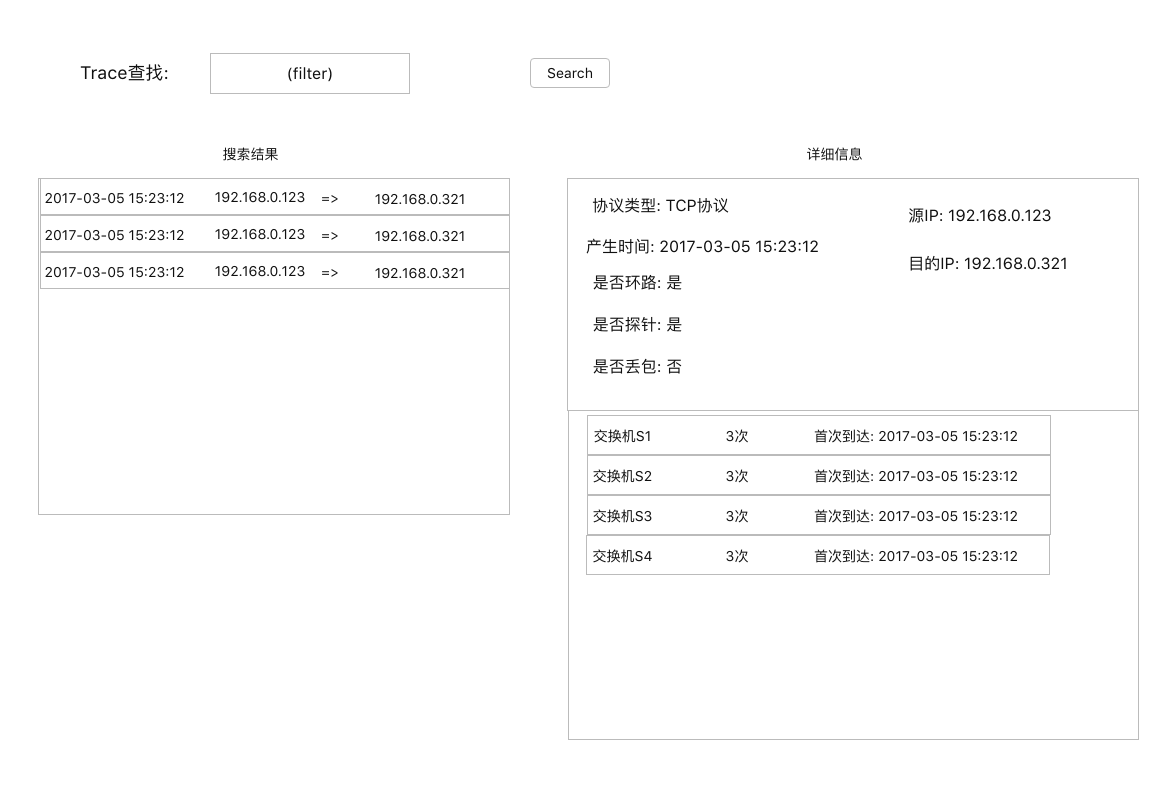
\includegraphics[width=0.9\textwidth]{../img/traffic_data_show.png}
    \captionof{figure}{Traffic data}
    \label{traffic_data_show}
\end{center}

\begin{center}
    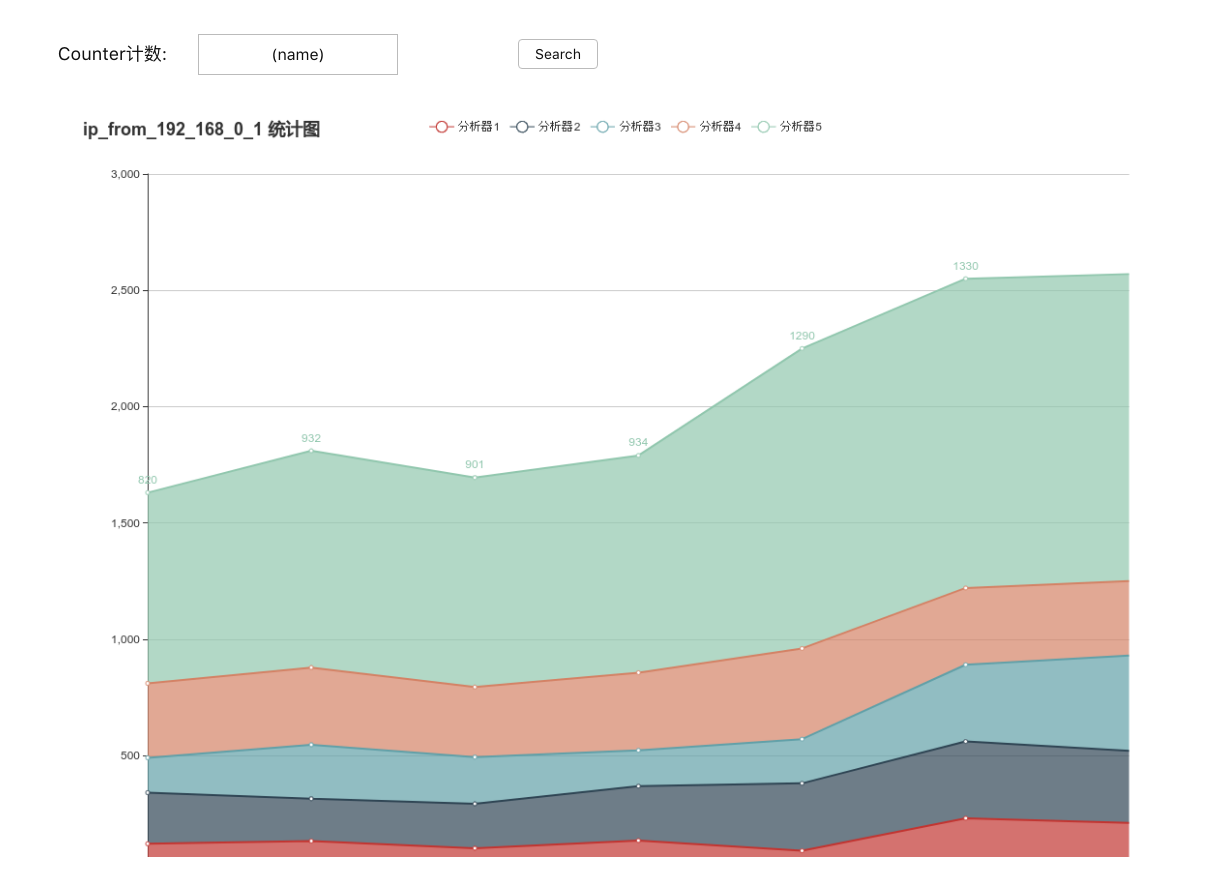
\includegraphics[width=0.9\textwidth]{../img/counter_data_show.png}
    \captionof{figure}{Counter data}
    \label{counter_data_show}
\end{center}

% }}}

% {{{ 技术选型
\subsection{技术选型}

此次系统设计, 技术选型主要包括分析器, 存储器, 以及控制器, 上层应用程序的设计.

根据对性能的不同要求, 结合开发进度做以下讨论. 在分析器中, 需要考虑大量的流量
涌来, 必须充分利用系统资源进行数据的接受和处理, 使用偏向底层的C/C++语言, 在控制器中,
只涉及简单的数据库查找与用户交互, 对性能要求不高, 故使用Python, 以实现迅速而
敏捷的开发.

对于本次的系统设计, 分工如下:
\begin{itemize}
    \setlength\itemsep{0.1em}
    \item 分析器采用C/C++完成
    \item 存储器可能选择MySQL作为存储
    \item 控制器主要通过Python实现, 期间某些静态库的编写使用C/C++完成.
            控制器的API接口采用HTTP协议交互, 最终的展示页面,
            功能配置也将在网页上进行操作, 其中, 图表展示打算使用开源的echarts.
\end{itemize}

% }}}

% {{{ 主要算法说明
\subsection{主要算法说明}\label{主要算法说明}

\textbf{检测环路算法}: 检测环路应该是几个算法中最为简单的一个,
只需要遍历数据流的所有节点, 如果不存在相同的节点,
那么可以认为此流量中没有环.

\textbf{检测丢包算法}: 查看路径的最后一跳是否与我们期望的最后一跳相同.
最后一跳的交换机 是无法直接计算得到的,
需要根据数据中心的网络拓扑进行分析.

\textbf{使用探针检测任意交换机的延迟}: 这是一个比较具有考量的方法.
使用了交换机的解封 和转发这一能力.

首先介绍如何实现一跳的探针: 假设我们想要将数据包p发往S,
我们首先根据p构造出\(p^{'}\) 其中\(p^{'}\)的目的IP为S,
而后将\(p^{'}\)发送出去, 当他到达交换机S后, 数据包中的
目的IP与S的IP相同, 则将数据包\(p^{'}\)进行解封操作, 将其还原为p,
再正常的转发规则 处理p.

实现了一跳的探针后, 我们可以考虑将探针进行拓展,
使其按找我们理想的路径进行传递, 方式也不难理解,
就是一层层的进行数据包封装, 这样数据包到达交换机被解封后, 就可以
根据内层的数据包进行正常转发了, 从而达到内层数据包所要去的地址中.
对于端到端的延迟, 例如我们想要知道\(S_{1}\)到\(S_{2}\)的往返延迟,
需要对原始数据包进行封装: 第一层, 以\(S_{1}\)的IP为目的IP, 第二层,
以\(S_{2}\)的IP为目的IP, 第三层, 再次将\(S_{1}\) 的IP作为目的IP.
数据包就会按照\(S_{1} => S_{2} => S_{1}\)的方式进行传递. 我们
可以通过此种方法得到粗略的往返延迟.

为什么说粗略呢, 这里,
并不是在交换机\(S_{1}\)上直接获取到了两次数据的间隔时间,
我们只能得到到达分析器的时间, 因为认为\(S_{1}\)到分析器来回路径是一致的,
因此可以 简单的使用分析器获得的两个时间相减得到粗略的往返延迟.

\textbf{定时器功能的实现}:

图\ref{hash_backet}介绍了定时功能的实现, 每经过1s三个数据桶进行一次状态转移,
以0s到1s的时间为例. 在此时间段内达到的数据包首先检查桶H0, 判断他的trace数据是否
属于H0, 如果属于, 则加入到桶H0中, 否则放置在桶H1中. 待1s结束, 到达1s到2s的时间段中,
我们将桶的状态进行转移, H0中的数据就可以作为慢路径进行处理,
因为桶中的每条trace数据已经包含了整整1s的数据包.

\begin{center}
    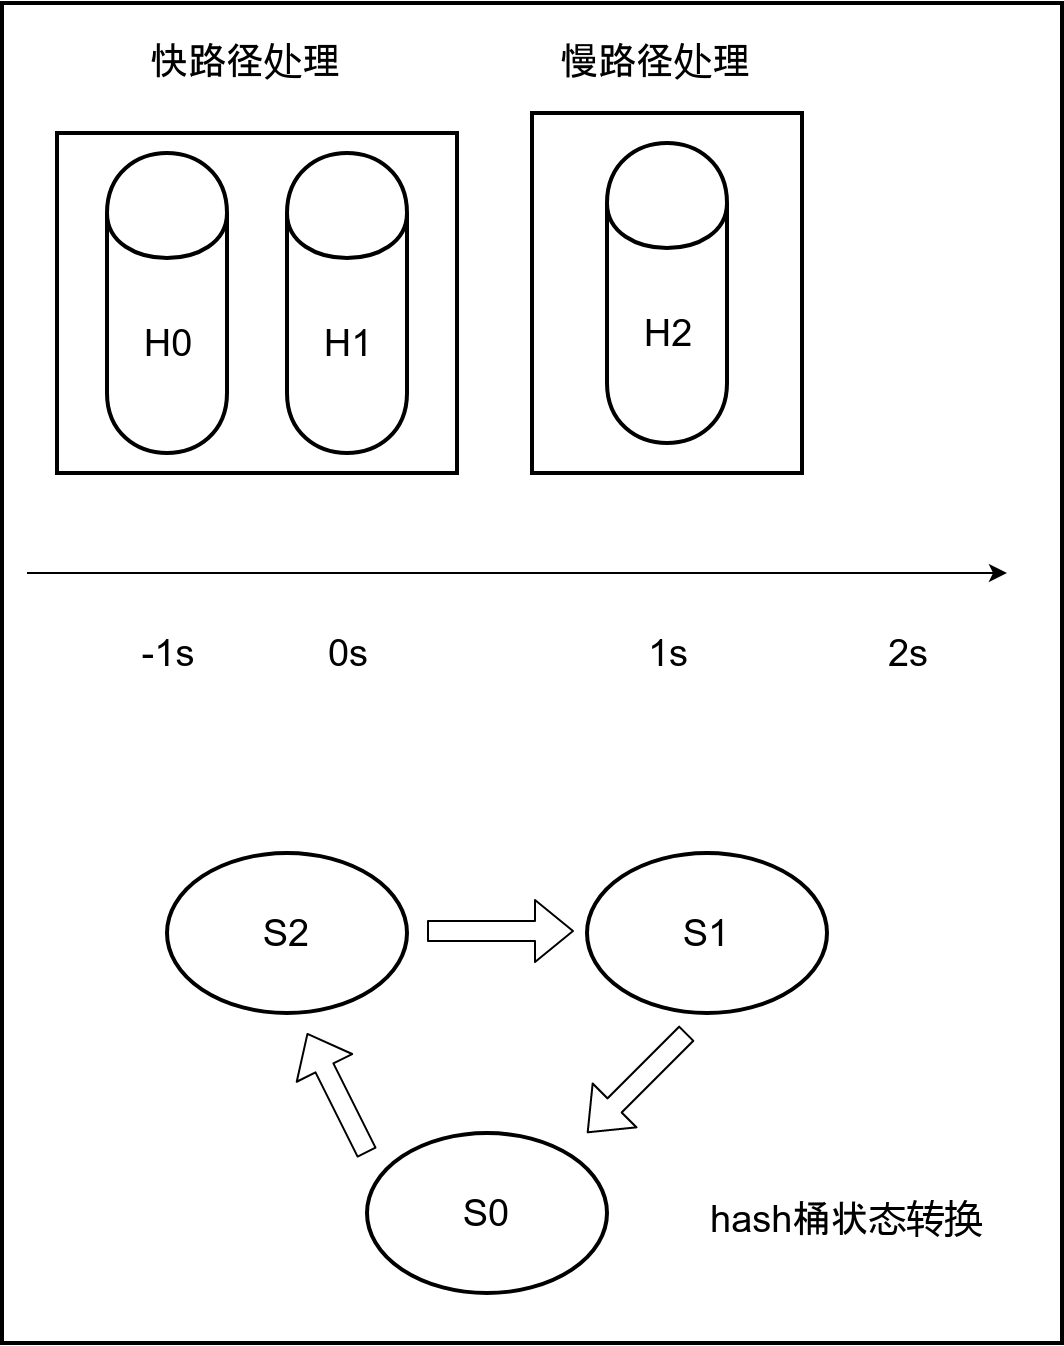
\includegraphics[width=0.8\textwidth]{../img/hash_backet.png}
    \captionof{figure}{hash backet}
    \label{hash_backet}
\end{center}
%}}}

% {{{ 主要数据结构说明
\subsection{主要数据结构说明}

\begin{center}
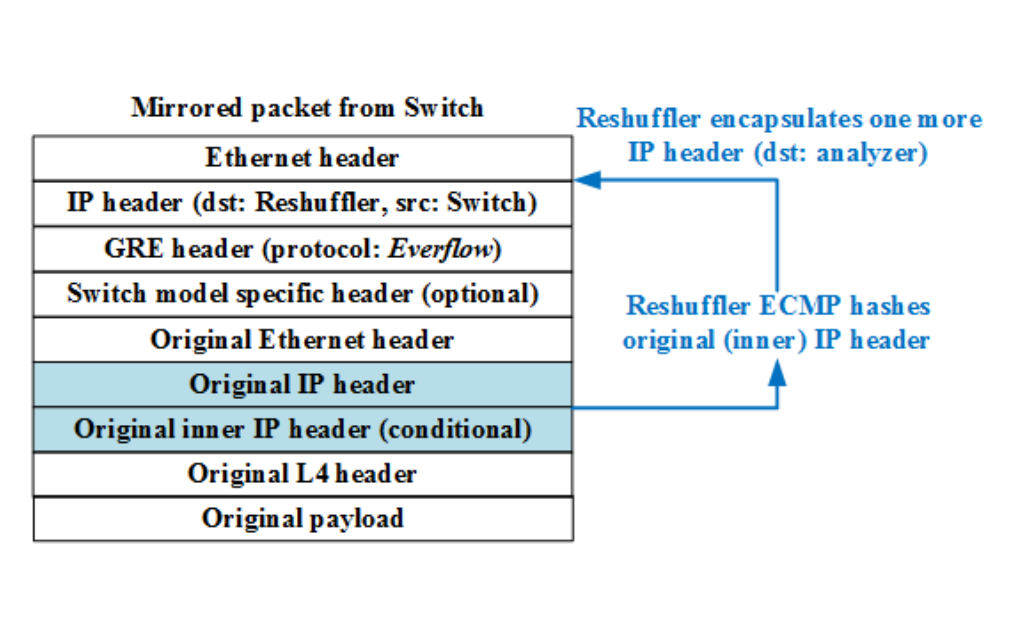
\includegraphics[width=0.6\textwidth]{../img/format_gre.png}
    \captionof{figure}{GRE packet}
\label{gre_packet}
\end{center}

对于到达分析器的数据包来说, 均是使用GRE(Generic Routing Encapsulation)
进行封装, GRE格式见图\ref{gre_packet}.

分析器中存储结构: 基于由于上述分析,
传入任意的分析器中的是一个个单独的数据包, 分析器中, 需要还原整条路径,
但是一条路径上数据包信息是相同的, 所以保存一份即可.
这里是还原后采用的trace路径表示形式.
另外对于每一条trace数据, 还具有一些元数据, 用以表示本trace数据的各种信息.

% {{{ traces数据

\begin{lstlisting}
/**
 * @brief  trace数据还有待讨论, 尤其是某些字段的长度
 *       以及是否为环, 是否丢包, 是否为探针数据
 */
typedef struct{
    uint32_t src_ip;    //源 IP 地址,32bits
    uint32_t dst_ip;    //目的 IP 地址,32bits
    uint16_t ip_ID;     //标识符,16 bits
    uint8_t protocol;   //协议字段,8 bits
}IP_PKT_KEY_T;

typedef struct{
    IP_PKT_KEY_T key;
    uint16_t pkt_size;   // 数据包大小

    uint32_t hop1_timestamp; // 收到第一个报文的时间戳:
                               // Timestamp记录收到报文的时间,
                               // 如果对于某一跳交换机超过1秒还没收到其报文,
                               // 则视为丢包

    uint16_t switch_id[5];      // 只保留交换机id
    uint16_t hop1_rcvd : 2;     // 交换机收到的报文数

    uint16_t used : 1;          // 以hash表进行存储,
                                // 记录hash表中的当前元素是否被占用.
    uint16_t rcvd : 5;
    uint16_t hop2_rcvd : 2;
    uint16_t hop3_rcvd : 2;
    uint16_t hop4_rcvd : 2;
    uint16_t hop5_rcvd : 2;
    uint16_t hop2_timestamp : 10;
    uint16_t hop3_timestamp : 10;
    uint16_t hop4_timestamp : 10;
    uint16_t hop5_timestamp : 10;
} PKT_TRACE_T;
\end{lstlisting}
% }}}

除此之外, 分析器中还有计数器, 记录每个规则下的trace数据个数.

在程序中, 需要经过快路径, 慢路径两个处理过程, 由快路径处理结束后, 进入


\subsubsection{存储器结构}

存储器中的结构: 使用关系型数据库进行存储.

存储路径的数据表分为三大部分:

\begin{itemize}
    \setlength\itemsep{0.1em}
    \item 第一部分是数据包原始信息, 包括数据包头部以及负载信息.
    \item 第二部分是每一跳的信息, 比如时间戳, 源MAC地址. 每个trace数据跳数不同,
            所以保存 时, 将所有跳的信息结合在一起存储.
    \item 第三部分是元数据信息, 表示这个trace信息是否有环, 是否丢包,
            是否为探针数据.
\end{itemize}


\begin{center}
    \captionof{table}{tbl\_traffic\_data}   % \caption{} 改为 \captionof{table}{}
    \begin{tabular}{llll}   \hline
    Field          & Type          & Comment                   \\ \hline
    id             & int(11)       &                           \\
    s\_ip          & int(11)       & 源IP                       \\
    d\_ip          & int(11)       & 目的IP                      \\
    protocal       & int(11)       & 协议类型                      \\
    generate\_time & timestamp     & 产生时间                      \\
    trace\_data    & varchar(1024) & trace数据信息, 保存为二进制字符串    \\
    fdate          & int(11)       & 存入日期, 如果数据量过大则使用索引 \\
    is\_loop       & int(11)       & 是否有环                      \\
    is\_drop       & int(11)       & 是否丢包                      \\
    is\_probe      & int(11)       & 是否为探针                    \\ \hline
    \end{tabular}
    \label{tbl_traffic_data}
\end{center}

存储计数器的数据表相对简单, 主要记录分析器ID, 计数值以及产生时间.

\begin{center}
    \captionof{table}{tbl\_counter}
    \label{tbl_counter}
    \begin{tabular}{lll} \hline
    Field          & Type          & Comment \\ \hline
    id             & int(11)       &         \\
    counter\_name  & varchar(1024) & 计数器名称   \\
    generate\_time & timestamp     & 数据产生时间  \\
    analyer\_id    & int(11)       & 分析器ID   \\
    cnt            & int(11)       & 计数值     \\
    fdate          & int(11)       & 数据产生日期  \\ \hline
    \end{tabular}
\end{center}


% }}}

\subsection{未来可进行的优化}

分析器中接受数据包时, 可以使用RSS(Receiver Size Scaling).
允许使用多个CPU 核来接受数据包.

使用专用的交换机与分析服务器, 充分利用硬件资源加速运算

\subsection{程序部署相关}

从理论上来说, 分析器, 存储器, 控制器以及最终展示的应用程序,
几个组件应该放置在 不同的服务器上, 为了开发方便,
暂时将其放在一台服务器上. 但这并不说明程序应该这样,
由于使用socket进行通讯, 所有的组件均可分开部署.
% }}}


% {{{ 结尾部分
\section{进度安排}

 下表\ref{schedule}为进度安排表.

\begin{centering}
\centering
    \captionof{table}{schedule}
    \label{schedule}

    \begin{tabular}{|l|p{0.17\textwidth}<{\centering}|p{0.48\textwidth}<{\centering}|} \hline
    起止日期              & 工作内容                                    & 备  注                                                          \\ \hline
    2018.1—2018.3         & 查阅文献, 了解需求, 撰写开题报告            & 除报告撰写, 论文翻译外, 老师提供了一组trace数据包, 初步进行了trace数据的解析, 为之后的分析器设计奠定基础 \\   \hline
    2018.3.10 ~ 2018.3.20 & 开题报告, 论文翻译完成                      & 程序架构的设计, 数据库设计, 主要数据结构的设计 \\ \hline
    2018.3.20 ~ 2018.3.31 & 编码实现                                    & 实现分析程序, 以及控制器的构建, 制作展示界面                        \\ \hline
    2018.4.1  ~ 2018.4.20 & 设计实现面向DCN网络的流量分析与故障检测方案 & 联调整个系统: 包括分析器, 存储器, 控制器及上层软件的设计                               \\    \hline
    2018.4.21 ~ 2018.4.30 & 进行测试与完善, 着手撰写毕业论文            & \\  \hline
    2018.5—2018.6         & 提交毕业论文, 完成论文答辩                  & \\ \hline

    \end{tabular}
\end{centering}


\section{主要参考文献}
\printbib
% }}}

\end{mdframed}
